\chapter{Proposed Methods for Online Stator Flux Linkage Estimation}\label{chapter3}
Since the measurements available from the SMs outputs are limited to stator current, electrical angular velocity, and position, it is not possible to directly estimate the flux linkage using a state observer designed based on the flux dynamics models in (\ref{eqn:2.9}) and (\ref{eqn:2.28}) (unobservable model). Section \ref{sec2:2.3.2} introduced a flux estimation method using a PI filter-based hybrid model to remove DC offsets occurring from purely integrating the stator flux linkage dynamics in (\ref{eqn:2.28}). However, the cutoff frequency of the filters degrades the transient estimation performance. Specifically, in control methods like FCS-MPC, using filters causes magnitude and phase distortions of the estimates due to filtered specific frequencies in the voltage input \cite{c3.2_1}. Section \ref{chap2:2.3.3} presented a method to estimate flux linkage by separating it into a linear flux term with nominal inductance and the remaining nonlinear flux term, extending this as an extended disturbance state to make it observable, and designing a state observer in the time domain. However, the flux estimation performance depends on the accuracy of the nominal parameter, and if it is inaccurate, the transient estimation performance may deteriorate.

In this chapter, two flux linkage estimators that can improve the estimation performance of existing flux estimators are proposed: the Extended State Observer-based Flux Linkage Estimator (ESO-FLE) and the Integration Error and Parameter Update-Based Flux Linkage Estimator (IE-PU-FLE). The main contributions of these estimators are (i) the development of an observable model based on the stator flux linkage dynamics, (ii) the design of the state observer in the time domain to prevent magnitude and phase distortion of the estimates caused by filters (i.e. LPF and HPF), especially in FCS-MPC switching method, and (iii) the reduction of dependence on nominal parameters used in the estimators, thereby improving transient estimation performance.

\section{Extended State Observer-based Flux Linkage Estimator \cite{c3.1_1}}\label{chap3:3.1}
The DOB-FLE in Section \ref{chap2:2.3.3} defines the nonlinear flux \(\Delta\boldsymbol{\psi}^{dq}_s\) as a disturbance step signal based on assumptions (A.2.1) and (A.2.2), and extends it as an additional state to be estimated. However, while this approach exhibits excellent estimation performance in steady state, its transient estimation performance is determined by the accuracy of the nominal inductance parameter ${\mathbf{L}^{dq}_{s,0}}$ used in the estimator. It means that the transient estimation performance depends on the parameter accuracy, and if the parameters are inaccurate, the nonlinear flux linkage \(\Delta\boldsymbol{\psi}^{dq}_s\) may be time-varying with a constant slope in transient state. In this section, to improve the transient estimation performance of the DOB-FLE, an extended state observer-based flux linkage estimator (ESO-FLE) is proposed. The key idea is to define the nonlinear flux \(\Delta\boldsymbol{\psi}^{dq}_s\) as a ramp signal with a constant slope and estimate it by extending this constant slope as an additional state to be estimated. 

The nonlinear flux linkage \(\Delta\boldsymbol{\psi}^{dq}_s\) (i.e. step disturbance signal) in Assumption (A.2.1) can be assumed as ramp disturbance signals
\begin{equation}\label{eqn:3.1}
\begin{aligned}
    \Delta\boldsymbol{\psi}^{dq}_s(t) = \left( \mathbf{L}^{dq}_{s} - \mathbf{L}^{dq}_{s,0} \right) \mathbf{i}^{dq}_s(t) + \boldsymbol{\psi}^{dq}_{pm} = \mathbf{c}^{dq}_s + \mathbf{l}^{dq}_s t,
\end{aligned}
\end{equation}
with unknown but constant slope \(\mathbf{l}^{dq}_s := (l^d_s,\ l^q_s)^\top\), which is extended the additional state to be estimated. The time derivative of the nonlinear flux linkage in (\ref{eqn:3.1}) can be expressed as 
\begin{align}\label{eqn:3.2}
\frac{d}{dt}\Delta{\boldsymbol{\psi}^{dq}_s} = \underbrace{\mathbf{\dot L}^{dq}_{s} \mathbf{i}^{dq}_s + \left( \mathbf{L}^{dq}_{s} - \mathbf{L}^{dq}_{s,0} \right) \mathbf{\dot i}^{dq}_s + \boldsymbol{\dot \psi}^{dq}_{pm}}_{\stackrel{(\ref{eqn:2.34})}= \mathbf{d}^{dq}_s(t)} = \mathbf{l}^{dq}_s(t),
\end{align}  
where, the time derivative of the constant slope $\mathbf{l}^{dq}_s$ in (\ref{eqn:3.2}) is represented as 
\begin{align}\label{eqn:3.3}
\frac{d}{dt}{\mathbf{l}^{dq}_s} = \underbrace{\mathbf{\ddot L}^{dq}_{s}\mathbf{i}^{dq}_s+2\mathbf{\dot L}^{dq}_{s} \dot{\mathbf{i}}^{dq}_s + \left( \mathbf{L}^{dq}_{s} - \mathbf{L}^{dq}_{s,0} \right) \mathbf{\ddot i}^{dq}_s + \boldsymbol{\ddot \psi}^{dq}_{pm}}_{=:  \mathbf{d}^{dq,l}_s(t) \rightarrow  0 \text{ as t} \rightarrow \infty},
\end{align}  
with the lumped disturbance vector $\mathbf{d}^{dq,l}_s:=(d^{d,l}_s,d^{q,l}_s)^\top$. Recalling Assumption (A.2.1), the lumped disturbance vector \(\mathbf{d}^{dq,l}_s\) can be upper bounded (all parameters and signals become constant in steady state) and becomes zero in steady state. Accordingly, the altered dynamic model is summarized as follows
\begin{equation}
\begin{aligned}\label{eqn:3.4_1}
\begin{cases}
\frac{d}{dt}{\bm{\psi}}^{dq}_s(t) = \mathbf{u}^{dq}_s(t) - R_s {\mathbf{L}^{dq}_{s,0}}^{-1} \left( \bm{\psi}^{dq}_s(t) - \Delta{\boldsymbol{\psi}^{dq}_s}(t) \right) - \omega_r(t) \mathbf{J} \bm{\psi}^{dq}_s(t) \\
\frac{d}{dt}{\Delta}{\boldsymbol{\psi}^{dq}_s}(t) = \mathbf{l}^{dq}_s(t) \\
\frac{d}{dt}{\boldsymbol{l}^{dq}_s}(t) = \mathbf{d}^{dq,l}_s(t) \\
\mathbf{i}_{dq}(t) = {\mathbf{L}^{dq}_{s,0}}^{-1} \left( \bm{\psi}^{dq}_s(t) - \Delta{\boldsymbol{\psi}^{dq}_s}(t) \right)
\end{cases}
\end{aligned}.
\end{equation}
Based on the dynamics in (\ref{eqn:3.4_1}), the state-space model 
\begin{align}\label{eqn:3.5_1}
&\left\{
\begin{aligned}
    \frac{d}{dt}{\mathbf{x}}(t) &= \mathbf{A}(\omega_r)\mathbf{x}(t) + \mathbf{B}\mathbf{u}(t) + \mathbf{d}(t)\\
    \mathbf{y}(t) &= \mathbf{C}\mathbf{x}(t)
\end{aligned}
\right.
\end{align}
with
\begin{equation*}
\begin{aligned}
\mathbf{x} &:= 
\begin{pmatrix}
\boldsymbol{\psi}^{dq}_s \\ \Delta\boldsymbol{\psi}^{dq}_s \\ \mathbf{l}^{dq}_s
\end{pmatrix}, \quad \mathbf{u} := \mathbf{u}^{dq}_s, \quad \mathbf{y} := \mathbf{i}^{dq}_s, \quad \mathbf{O}_{2\times2} := \begin{bmatrix}
0  & 0\\
0 & 0
\end{bmatrix}, \quad \mathbf{I}_{2\times2} := \begin{bmatrix}
1  & 0\\
0 & 1
\end{bmatrix}, \\
\mathbf{A}(\omega_r) &:= 
\begin{bmatrix}
-R_s {\mathbf{L}^{dq}_{s,0}}^{-1} - \omega_r \mathbf{J} & R_s {\mathbf{L}^{dq}_{s,0}}^{-1} & \mathbf{O}_{2\times2} \\
\mathbf{O}_{2\times2} & \mathbf{O}_{2\times2} & \mathbf{I}_{2\times2} \\
\mathbf{O}_{2\times2} & \mathbf{O}_{2\times2} & \mathbf{O}_{2\times2}
\end{bmatrix}, \mathbf{B} := \begin{bmatrix}
\mathbf{I}_{2\times2} \\
\mathbf{O}_{2\times2} \\
\mathbf{O}_{2\times2}
\end{bmatrix}, \mathbf{C} := 
\begin{bmatrix}
{\mathbf{L}^{dq}_{s,0}}^{-1} \\ -{\mathbf{L}^{dq}_{s,0}}^{-1} \\ \mathbf{O}_{2\times2}
\end{bmatrix}^\top, \\
\mathbf{d} &:= \begin{bmatrix}
    \mathbf{O}_2 & \mathbf{O}_2 & \mathbf{d}^{dq,l}_s
\end{bmatrix}^\top, \quad \mathbf{O}_2 := \begin{bmatrix}
    0 & 0
\end{bmatrix}^\top,
\end{aligned}
\end{equation*}
where $\mathbf{x}$ represents the state vector, $\mathbf{u}$ denotes the input vector, $\mathbf{y}$ represents the output vector and $\mathbf{d}$ is the lumped disturbance vector. The matrix $\mathbf{A}(\omega_r)$ is the system matrix with respect to $\omega_r$, $\mathbf{B}$ is the input matrix, and $\mathbf{C}$ is the output matrix. 

To analyze whether the states of the dynamic system in (\ref{eqn:3.4_1}) are fully observable, the observability matrix is analyzed (for constant $\omega_r$), i.e.
\begin{equation}\label{eqn:3.6_1}
\mathbf{\mathcal{O}}(\omega_r) = \begin{bmatrix}
\mathbf{C} \\
\mathbf{CA}(\omega_r) \\
\vdots \\
\mathbf{CA}(\omega_r)^5
\end{bmatrix},
\end{equation}
which is evaluated using the first three rows of $\mathbf{\mathcal{O}}(\omega_r)$ for simplicity. Consequently, the observability matrix has a full rank (i.e., $\mathbf{\mathcal{O}}(\omega_r) = 6$) if $\omega_r \neq 0$, and the state $\mathbf{x}$ is (locally) fully observable. The method for designing an observer for flux estimation is the same as that mentioned in DOB-FLE.

ESO-FLE assumes the nonlinear flux as a time-varying ramp disturbance signal with a constant slope and extends this slope as an additional state to be estimated. This approach improves transient estimation performance by considering the rapidly changing current behavior or additional disturbance signals caused by incorrect nominal inductance. However, if noise or uncertainties exist in the extended states, the estimates become highly sensitive to the observer's gain matrix, so it is crucial to select the optimal gain accordingly.

\section{Integration Error Estimation and Parameter Update-Based Flux Linkage Estimator} \label{sec3:3.2.1}
As above mentioned, purely integrating the voltage model in (\ref{eqn:2.28}) results in the actual flux linkage in the ($\alpha$,$\beta$)-reference frame and the integration errors caused by discrepancies. Therefore, this section presents (i) an observable model that can directly estimate these integration errors and proposes a state observer in the time domain that directly compensates for these integration errors from the integration results. Additionally, since the selection of the nominal inductance used in the observer determines the transient estimation performance, this section proposes (ii) a method to update this value to reflect the actual value, thereby improving transient estimation performance. Furthermore, (iii) an adaptive observer that is robust to parameter variations is suggested.

\subsection{Flux Linkage Estimation based on Integration Error Estimation}
\subsubsection{Flux Model Reformulation for Integration Error Estimation}
The pure integration results of the voltage model in (\ref{eqn:2.28}) can be physically separated into the actual flux linkage term $\boldsymbol{\psi}^{\alpha\beta}_s$ and the integration error term $\boldsymbol{O}^{\alpha\beta}_s$, which is accumulated due to input and initial value errors \cite{c3.2_1}, i.e.
\begin{align}\notag
\bm{\psi}^{\alpha\beta}_{s,\text{int}}(t) &= \int_{0}^{t} \left( \bm{u}^{\alpha\beta*}_{s}(\tau) - \hat R_s \bm{i}^{\alpha\beta}_s(\tau) \right) d\tau + \bm{\psi}^{\alpha\beta}_{s,\text{int}}(0)
\\\label{eqn:3.4}
&= \boldsymbol{\psi}^{\alpha\beta}_s(t) + \boldsymbol{O}^{\alpha\beta}_s(t) 
\end{align}
with $\boldsymbol{\psi}^{\alpha\beta}_s := (\psi^{\alpha}_s, \psi^{\beta}_s)^T$ and $\boldsymbol{O}^{\alpha\beta}_s := (O^{\alpha}_s, O^{\beta}_s)^T$. The $d$-$q$ axis flux linkages in (\ref{eqn:2.10}) can be rearranged by expressing them as
\begin{align}\notag
\boldsymbol\psi^{dq}_s(t) 
&= 
\mathbf{L}^{dq}_s(t)
\mathbf{i}^{dq}_s(t)
+
\boldsymbol{\psi}^{dq}_{pm}(t) \\
&= 
L^q_s(t)\boldsymbol{i}^{dq}_s(t)
+
\begin{bmatrix}
    \underbrace{(L^d_s(t) - L^q_s(t))i^d_s(t) + \psi_{pm}(t)}_{=:\Delta\psi^d_s(t)} \\
    0
\end{bmatrix}\label{eqn:3.5}
\end{align}
using only the $q$-axis inductance as a proportional constant, where $\Delta\psi^d_s$ denotes the $d$-axis nonlinear flux linkage caused by the saliency of the SMs rotor and the permanent magnetic flux linkage. 

By applying the inverse of the simplified Park transformation in (\ref{eqn:2.8}) to (\ref{eqn:3.5}), the stator flux linkage vector in the ($\alpha$,$\beta$)-reference frame can be obtained as follows
\begin{align}\label{eqn:3.6a}
\boldsymbol{\psi}^{\alpha\beta}_s(t) &= L^q_s(t) \mathbf{i}^{\alpha\beta}_s(t) + 
\mathbf{P}(\theta_r)
\Delta \psi^{d}_s(t)\\\label{eqn:3.6b}
&= \hat{L}^q_s(t) \mathbf{i}^{\alpha\beta}_s(t) + 
 \underbrace{(L^q_s(t) -\hat{L}^q_s(t))\mathbf{i}_{\alpha\beta}(t) + \mathbf{P}(\theta_r)
\Delta \psi^{d}_s(t)}_{=:\Delta \boldsymbol{\psi}^{\alpha \beta}_s(t)} ,
\end{align}
where $\hat{L}_q$ denotes the estimate of $L_q$, $\mathbf{P}(\theta_r) := [\cos\theta, \sin\theta]^\top$ represents the rotational vector, and $\Delta \boldsymbol{\psi}^{\alpha \beta}_s := (\Delta \psi^\alpha_s,\Delta \psi^\beta_s)^\top$ denotes the nonlinear flux linkage vector rotating in circular motion (only in steady state) in the ($\alpha$,$\beta$)-reference frame, which is caused by inaccurate $q$-axis static (average) inductance $L^q_s$ and $\Delta\psi^d_s$ in (\ref{eqn:3.5}). Substituting (\ref{eqn:3.6b}) into (\ref{eqn:3.4}) leads to the altered integration results
\begin{equation}\label{eqn:3.7}
\boldsymbol{\psi}^{\alpha\beta}_{s,\text{int}}(t) = \hat{L}^q_s(t) \mathbf{i}^{\alpha\beta}_s(t) + 
\Delta \boldsymbol{\psi}^{\alpha \beta}_s(t) + \mathbf{O}^{\alpha\beta}_s(t).
\end{equation}
Computing the time derivative of the rotating nonlinear flux $\Delta \boldsymbol{\psi}^{\alpha \beta}_s$ in (\ref{eqn:3.6b}) directly yields
\begin{equation}\label{eqn:3.8}
\begin{aligned}
\frac{d}{dt}{\boldsymbol{\Delta \psi}}^{\alpha\beta}_s(t) &= \omega_r(t) \mathbf{J}\underbrace{\left(\mathbf{P}(\theta_r)\Delta \psi^{d}_s(t) + \tilde{L}^q_s(t)\mathbf{i}^{\alpha\beta}_s(t)\right)}_{\stackrel{(\ref{eqn:3.6b})}=\Delta\boldsymbol{\psi}^{\alpha\beta}_s}\\
&+\underbrace{\tilde{L}^q_s(t)\left(\dot{\mathbf{ i}}^{\alpha\beta}_s(t)-\omega_r(t) \mathbf{J}\mathbf{i}^{\alpha\beta}_s(t)\right) + \dot{\tilde{L}}^q_s(t)\mathbf{i}^{\alpha\beta}_s(t) + \mathbf{P}(\theta_r) \Delta \dot\psi^{ d}_s(t)}_{=:\mathbf{d}^{\alpha\beta,\psi}_{s}(t)}
\\
&= \omega_r(t) \mathbf{J} \Delta \boldsymbol{\psi}^{\alpha\beta}_s(t) + \mathbf{d}^{\alpha\beta,\psi}_{s}(t)
\end{aligned}
\end{equation}
in the $(\alpha,\beta)$-reference, where \( \tilde{L}^q_s :=  L^q_s-\hat{L}^q_s \) denotes the parameter estimation error, and \(\mathbf{d}^{\alpha\beta,\psi}_{s} := (d^{\alpha,\psi}_{s}, d^{\beta,\psi}_{s})^\top\) represents the lumped disturbance vector caused by the inductance parameter variation and nonlinear flux $\Delta\psi^d_s$ in (\ref{eqn:3.5}). The physical behaviors of the lumped disturbance $\mathbf{d}^{\alpha\beta,\psi}_{s}$ in (\ref{eqn:3.8}) can be explained by the following assumptions.

\textbf{Assumption (A.3.1)} The dynamics system in (\ref{eqn:2.5}) are bounded-input-bounded-output (BIBO) stable and the lumped disturbance vector $\mathbf{d}^{\alpha\beta,\psi}_{s}$ in (\ref{eqn:3.8}) is upper bounded by
\begin{equation}\notag
   ||\mathbf{d}^{\alpha\beta,\psi}_{s} || \stackrel{(\ref{eqn:3.8})}\leq  ||\tilde{L}^q_s|| ||\dot{\mathbf{ i}}^{\alpha\beta}_s ||+\left(||\omega_r|| +||\dot{\tilde{L}}^q_s|| \right) ||\mathbf{i}^{\alpha\beta}_s|| + ||\Delta \dot\psi^{ d}_s||.
\end{equation}

\textbf{Assumption (A.3.2)} In view of Assumption (A.2.1) and Assumption (A.2.2), all parameters and signals in the ($d$,$q$)-reference frame become constant, and their time derivatives become zero (only) in steady state. Meanwhile, the time derivative of the current vector in the ($\alpha$,$\beta$)-reference frame is always in a circular motion with the electrical angular velocity $\omega_r$ (only) in steady state \cite{c3.2_7}. Thus, the lumped disturbance vector $\mathbf{d}^{\alpha\beta,\psi}_{s} $ in the ($\alpha$,$\beta$)-reference frame becomes the zero vector \(\mathbf{O}_2\), i.e.
\begin{align}\notag
    \mathbf{d}^{\alpha\beta,\psi}_s \rightarrow \mathbf{O}_2 \quad \left(\dot{\tilde{L}}^q_s \rightarrow 0, \quad \Delta\dot{\psi}^d_s \rightarrow 0, \quad \dot{\mathbf{i}}^{\alpha\beta}_s \rightarrow \omega_r \mathbf{J} \mathbf{i}^{\alpha\beta}_s \text{ as } t \rightarrow \infty \right)
\end{align}

Likewise, computing the time derivative of the integration error vector $\mathbf{O}^{\alpha\beta}_s$ in (\ref{eqn:3.7}) directly yields
\begin{equation}\label{eqn:3.9}
\frac{d}{dt}{\mathbf{O}}^{\alpha\beta}_s(t) = \mathbf{d}^{\alpha\beta,o}_{s}(t)
\end{equation}
in the $(\alpha,\beta)$-reference with the disturbance vector of integration error $\mathbf{d}^{\alpha\beta,o}_{s} := (d^{\alpha,o}_{s}, d^{\beta,o}_{s})^\top$ (only) in transient state, which can be explained by the following assumption.

\textbf{Assumption (A.3.3)} In view of Assumption (A.3.1), the integration error vector ${\mathbf{d}}^{\alpha\beta,o}_s$ is bounded and consists of low-frequency components such as DC offsets in the ($\alpha$,$\beta$)-reference frame. Therefore, the time derivative of the integration error becomes zero (only) in the steady state (i.e., $\mathbf{d}^{\alpha\beta,o}_s \rightarrow \mathbf{O}_2$ as $t \rightarrow \infty$). The concepts of these assumptions are illustrated in Fig. \ref{Fig:3.1a}. 

Considering Assumption (A.3.1)$-$(A.3.2), the output in (\ref{eqn:3.7}) and the dynamics in (\ref{eqn:3.8}) and (\ref{eqn:3.9}) are summarized as follows
\begin{equation}
\begin{aligned}\label{eqn:3.10}
\begin{cases}
\frac{d}{dt}{\Delta \boldsymbol{\psi}}^{\alpha\beta}_s(t) = \omega_r(t) \mathbf{J} \Delta \boldsymbol{\psi}^{\alpha\beta}_s(t) + \mathbf{d}^{\alpha\beta,\psi}_{s}(t) \\
\frac{d}{dt}{\mathbf{O}}^{\alpha\beta}_s(t) = \mathbf{d}^{\alpha\beta,o}_{s}(t) \\
\boldsymbol{\psi}^{\alpha\beta}_{s,\text{int}}(t) = \hat{L}^q_s(t) \mathbf{i}^{\alpha\beta}_s(t) + 
\Delta \boldsymbol{\psi}^{\alpha \beta}_s(t) + \mathbf{O}^{\alpha\beta}_s(t)
\end{cases}
\end{aligned}.
\end{equation}
\begin{figure}[t]
    \centering
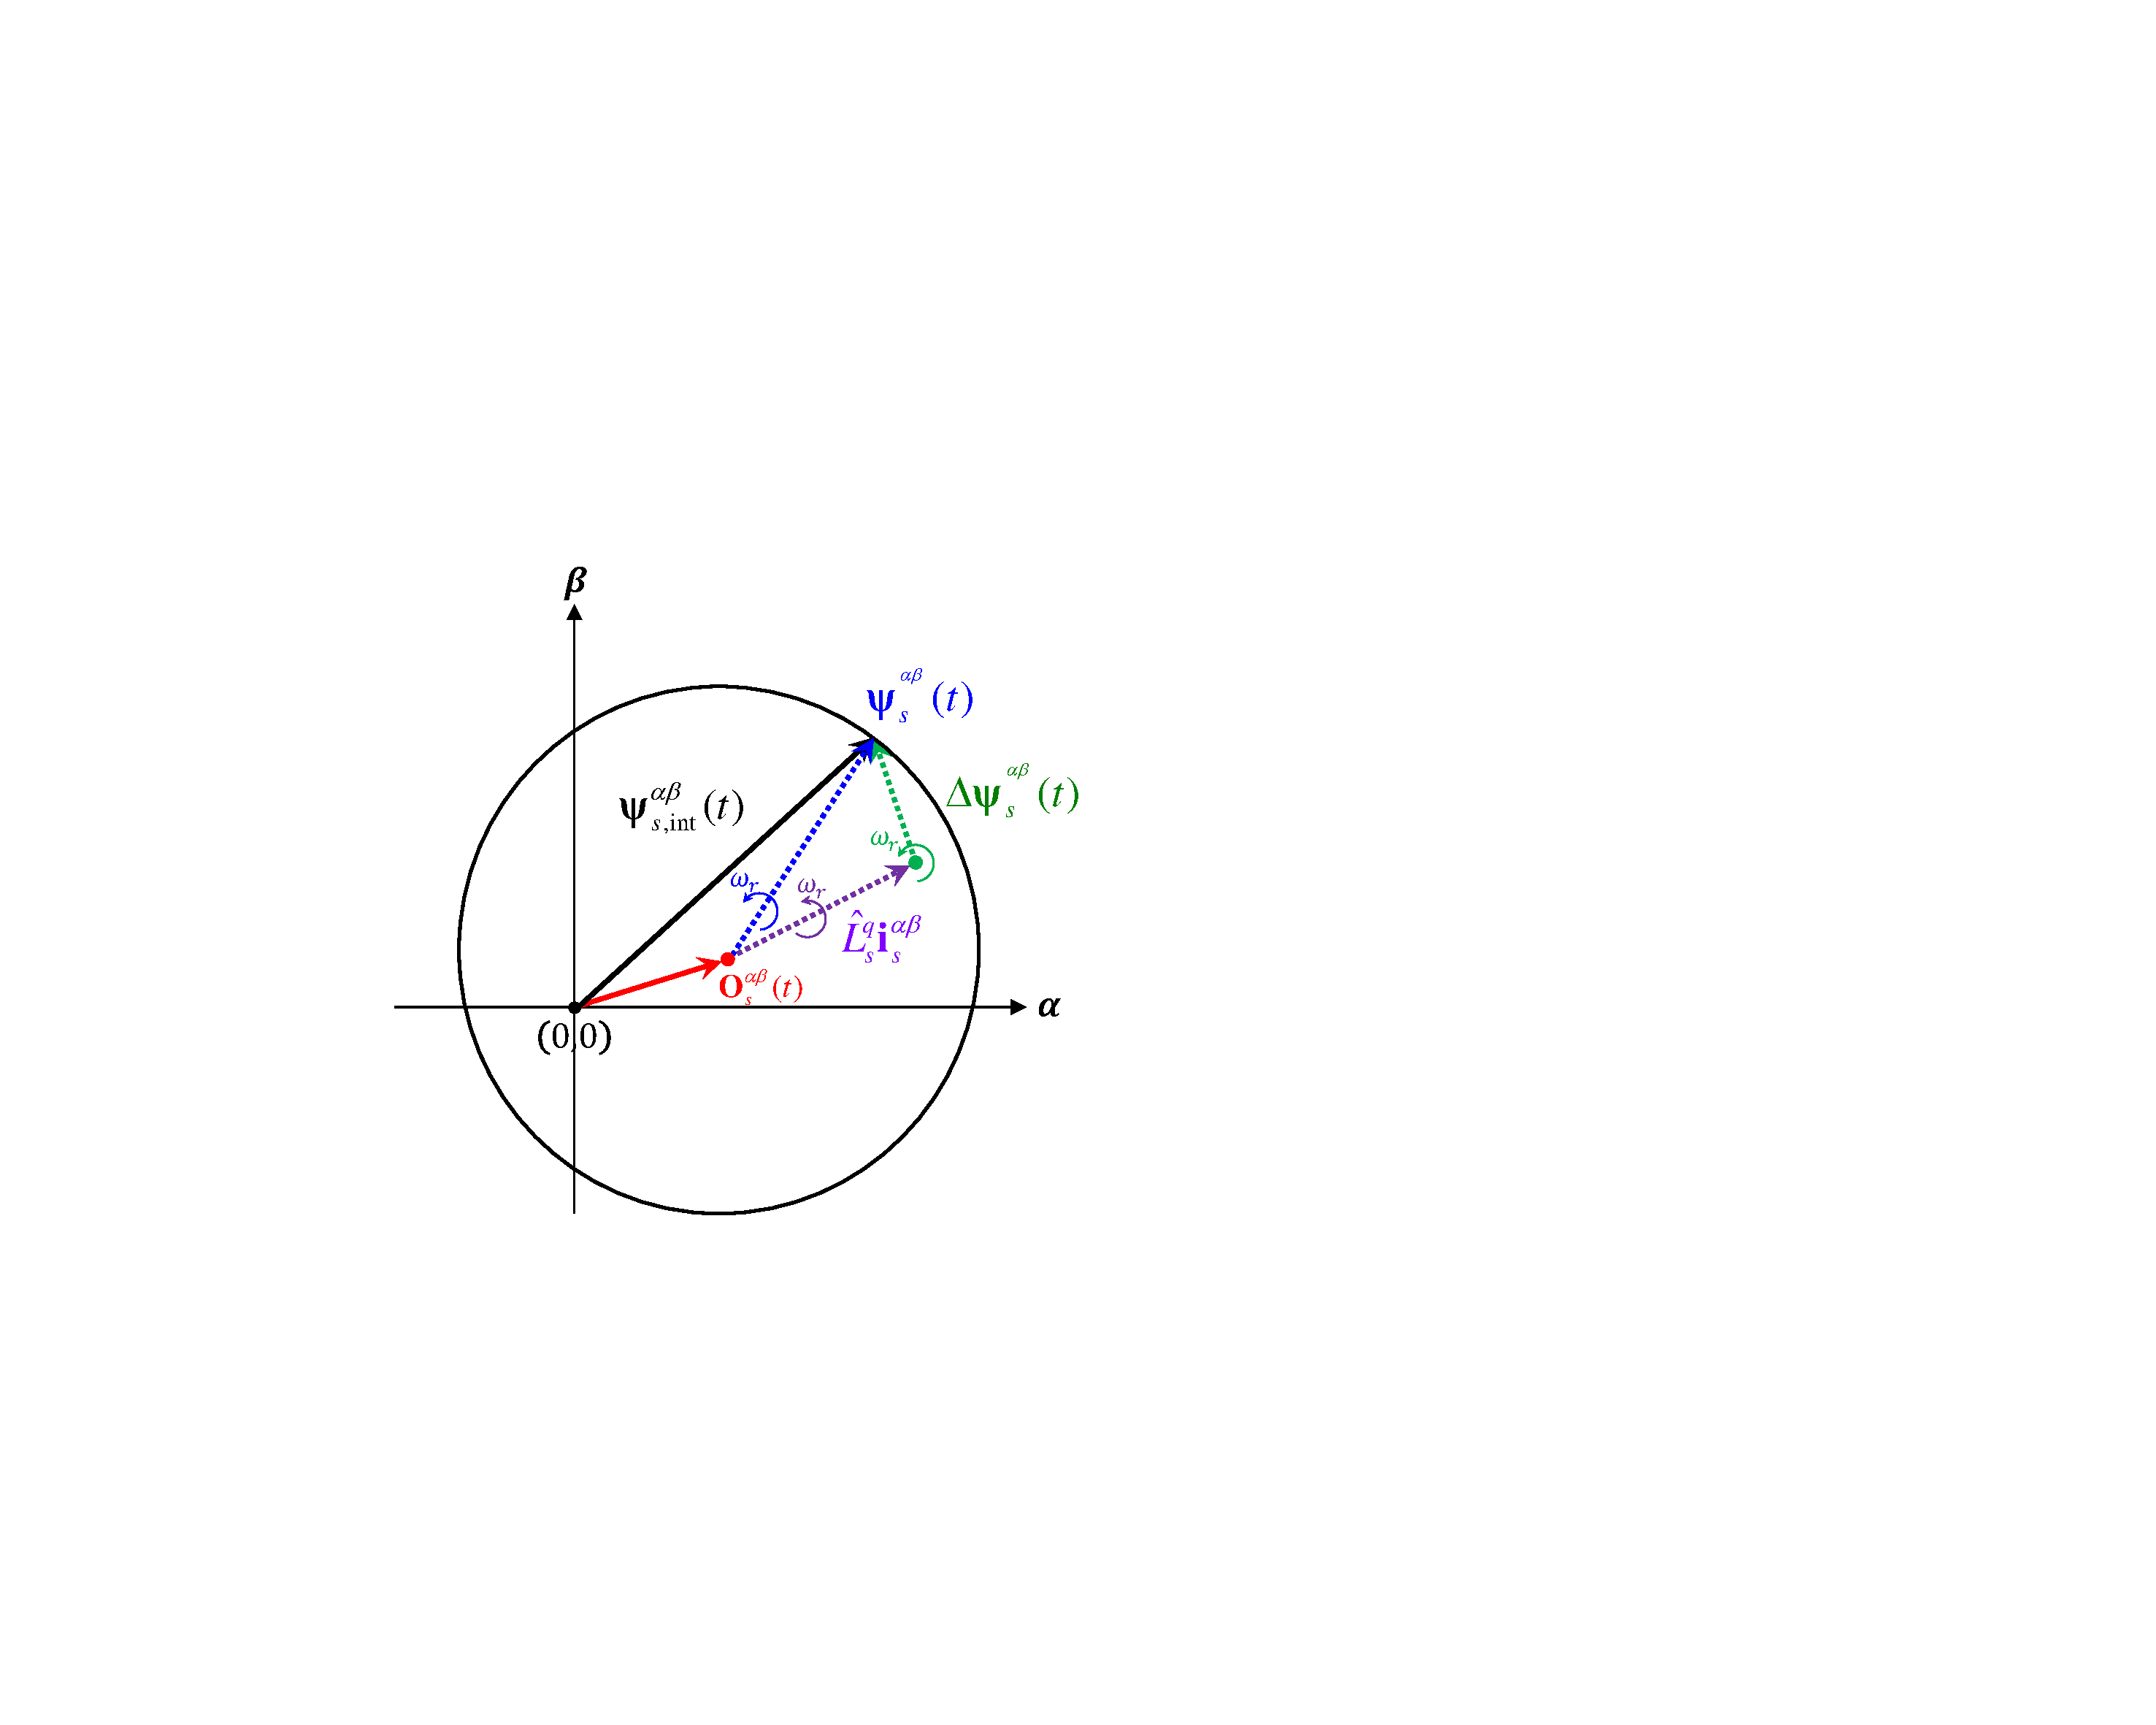
\includegraphics[scale=0.50]{chapters/Fig3.1a.pdf}
    \caption{Components of the integration result $\boldsymbol{\psi}^{\alpha\beta}_{s,\text{int}}$ in steady state.}
    \label{Fig:3.1a}
\end{figure}

\subsubsection{Observable State-Space Model}
By estimating $\Delta\boldsymbol{\psi}^{\alpha\beta}_s$ and ${\mathbf{O}}^{\alpha\beta}_s$ and compensating for the integration error vector ${\mathbf{O}}^{\alpha\beta}_s$ from the integration result vector of (\ref{eqn:3.7}), the stator flux linkage vector $\boldsymbol{\psi}^{\alpha\beta}_s$ can be estimated. Thus, based on (\ref{eqn:3.10}), the state-space model is expressed as
\begin{equation}\label{eqn:3.11}
\left\{
\begin{aligned}
    \frac{d}{dt} \mathbf{x}(t) &= \mathbf{A}(\omega_r) \mathbf{x}(t) + {\mathbf{d}_{t}}(t) \\
    \mathbf{y}(t) &= \mathbf{C} \mathbf{x}(t) + \mathbf{\Psi}(t) \theta(t)
\end{aligned}
\right.
\end{equation}
with
\begin{equation*}
\begin{aligned}
 \mathbf{x} &:= 
\begin{pmatrix}
\boldsymbol{\Delta \psi}^{\alpha\beta}_s \\
\mathbf{O}^{\alpha\beta}_s
\end{pmatrix},
\quad
\mathbf{y} := \boldsymbol{\psi}^{\alpha\beta}_{s,\text{int}}, \quad
\mathbf{d}_t := 
\begin{bmatrix}
\mathbf{d}^{\alpha\beta,\psi}_{s} \\ \mathbf{d}^{\alpha\beta,o}_{s}
\end{bmatrix}, \quad \mathbf{\Psi} := \mathbf{i}_{\alpha\beta},
\quad
\theta:= \hat L_q,
\\
\mathbf{A}(\omega_r) &:= 
\begin{bmatrix}
\omega_r \mathbf{J} & \mathbf{O}_{2\times 2} \\
\mathbf{O}_{2\times 2} & \mathbf{O}_{2\times 2}
\end{bmatrix},
\quad
\mathbf{C} := 
\begin{bmatrix}
\mathbf{I}_{2\times 2} & \mathbf{I}_{2\times 2}
\end{bmatrix}, \quad \mathbf{O}_{2\times2} := \begin{bmatrix}
0  & 0\\
0 & 0
\end{bmatrix}, \quad \mathbf{I}_{2\times2} := \begin{bmatrix}
1  & 0\\
0 & 1
\end{bmatrix},
\end{aligned}
\end{equation*}
where \( \mathbf{x} \) represents the state vector, \( \mathbf{y} \) is the output vector, \( \mathbf{d} \) is the disturbance vector, \( \mathbf{C} \) is the output matrix, \( \mathbf{A}(\omega_r) \) is the time-varying system matrix, \(\mathbf{\Psi}\) represents the current vector in the ($\alpha$,$\beta$)-reference frame, and \(\theta\) denotes an estimate of the $q$-axis inductance parameter, which is updated online to reduce the magnitude of the disturbance vector \(\mathbf{d}\) and improve transient estimation performance. These matrices and vectors are all piecewise continuous and uniformly bounded in time.

To verify whether the dynamic system in (\ref{eqn:3.10}) is observable or not, the observability matrix of the state-space model in (\ref{eqn:3.10}) is given by
\begin{equation}\label{eqn:3.12}
\mathcal{O}(\omega_r) = \begin{bmatrix}
\mathbf{C} \\
\mathbf{C}\mathbf{A}(\omega_r) \\
\mathbf{C}\mathbf{A}(\omega_r)^2 \\
\mathbf{C}\mathbf{A}(\omega_r)^3
\end{bmatrix} = \begin{bmatrix}
\mathbf{I}_{2\times2}& \mathbf{I}_{2\times2} \\
\omega_r \mathbf{J} & \mathbf{O}_{2\times2} \\
(\omega_r \mathbf{J})^2 & \mathbf{O}_{2\times2} \\
(\omega_r \mathbf{J})^3 & \mathbf{O}_{2\times2}
\end{bmatrix},  
\end{equation}
which has a full rank (i.e., \(\mathcal{O}(\omega_r) = 4\)) except for \(\omega_r = 0\), so \(\mathbf{x}\) is fully observable at all constant nonzero electrical angular velocities (as it is slowly varying compared to electrical quantities), similar to the DOB-FLE and ESO-FLE methods. 

\subsubsection{A Liner State Observer Design}
A linear state observer for the state-space model in (\ref{eqn:3.10}) is designed as follows
\begin{equation}\label{eqn:3.13}
\left\{
\begin{aligned}
    \frac{d}{dt} \hat{\mathbf{x}}(t) &= \mathbf{A}(\omega_r) \hat{\mathbf{x}}(t) + \mathbf{F}(\omega_r) \left( \mathbf{y}(t) - \mathbf{C} \hat{\mathbf{x}} - \mathbf{\Psi}(t) \theta(t) \right) \\
    \hat{\mathbf{y}}(t) &= \mathbf{C} \hat{\mathbf{x}}(t) + \mathbf{\Psi}(t) \theta(t)
\end{aligned}
\right.
\end{equation}
where \(\mathbf{\hat{x}}\) and \(\mathbf{\hat{y}}\) represent the estimates of \(\mathbf{x}\) and \(\mathbf{y}\), respectively. The observer gain matrix \(\mathbf{F}(\omega_r) \in \mathbb{R}^{4 \times 2}\) has to be determined with the electrical angular velocity and $\mathbf{A}(\omega_r)$ (i.e. speed-dependant). The dynamic system in (\ref{eqn:3.11}) represents a MIMO (Multi-Input-Multi-Output) system with more variables to estimate than the output equations of the observer. Therefore, \(\mathbf{F}(\omega_r)\) must be designed using eigenstructure assignment as described in \cite{c3.2_2} or robust pole assignment as detailed in \cite{c3.2_3} to accurately place the four closed-loop poles of the observer in (\ref{eqn:3.13}), thus achieving the desired bandwidth of the stable eigenvalues (equivalent to the poles) of the closed-loop observer matrix \(\mathbf{A}(\omega_r) - \mathbf{F}(\omega_r)\mathbf{C}\). In this study, to determine the observer gain matrix \( \mathbf{F}(\omega_r) \), a robust pole assignment method in \cite{c3.2_3} is utilized to place the system poles at the desired (stable) eigenvalues (i.e. establishing a Hurwitz observer matrix \(\mathbf{A}(\omega_r) - \mathbf{F}(\omega_r)\mathbf{C}\) with eigenvalues having negative real parts), which can be calculated using the MATLAB command \texttt{place}. 

Accordingly, by subtracting (\ref{eqn:3.11}) from (\ref{eqn:3.13}), the estimation error dynamics
\begin{equation}\label{eqn:3.14}
\frac{d}{dt} {\mathbf{\tilde{x}}}(t) = \left[ \mathbf{A}(\omega_r) - \mathbf{F}(\omega_r)\mathbf{C} \right] {\mathbf{\tilde{x}}}(t)- {\mathbf{d}_{t}}(t).
\end{equation}
with estimation error $\mathbf{\tilde{x}}:= \mathbf{\hat x}-\mathbf{ x}$ are exponentially stable as the disturbance vector \( \mathbf{d}_{t} \) eventually becomes zero in steady state based on Assumption (A.3.1)$-$(A.3.3).

\begin{figure}[t]
    \centering
    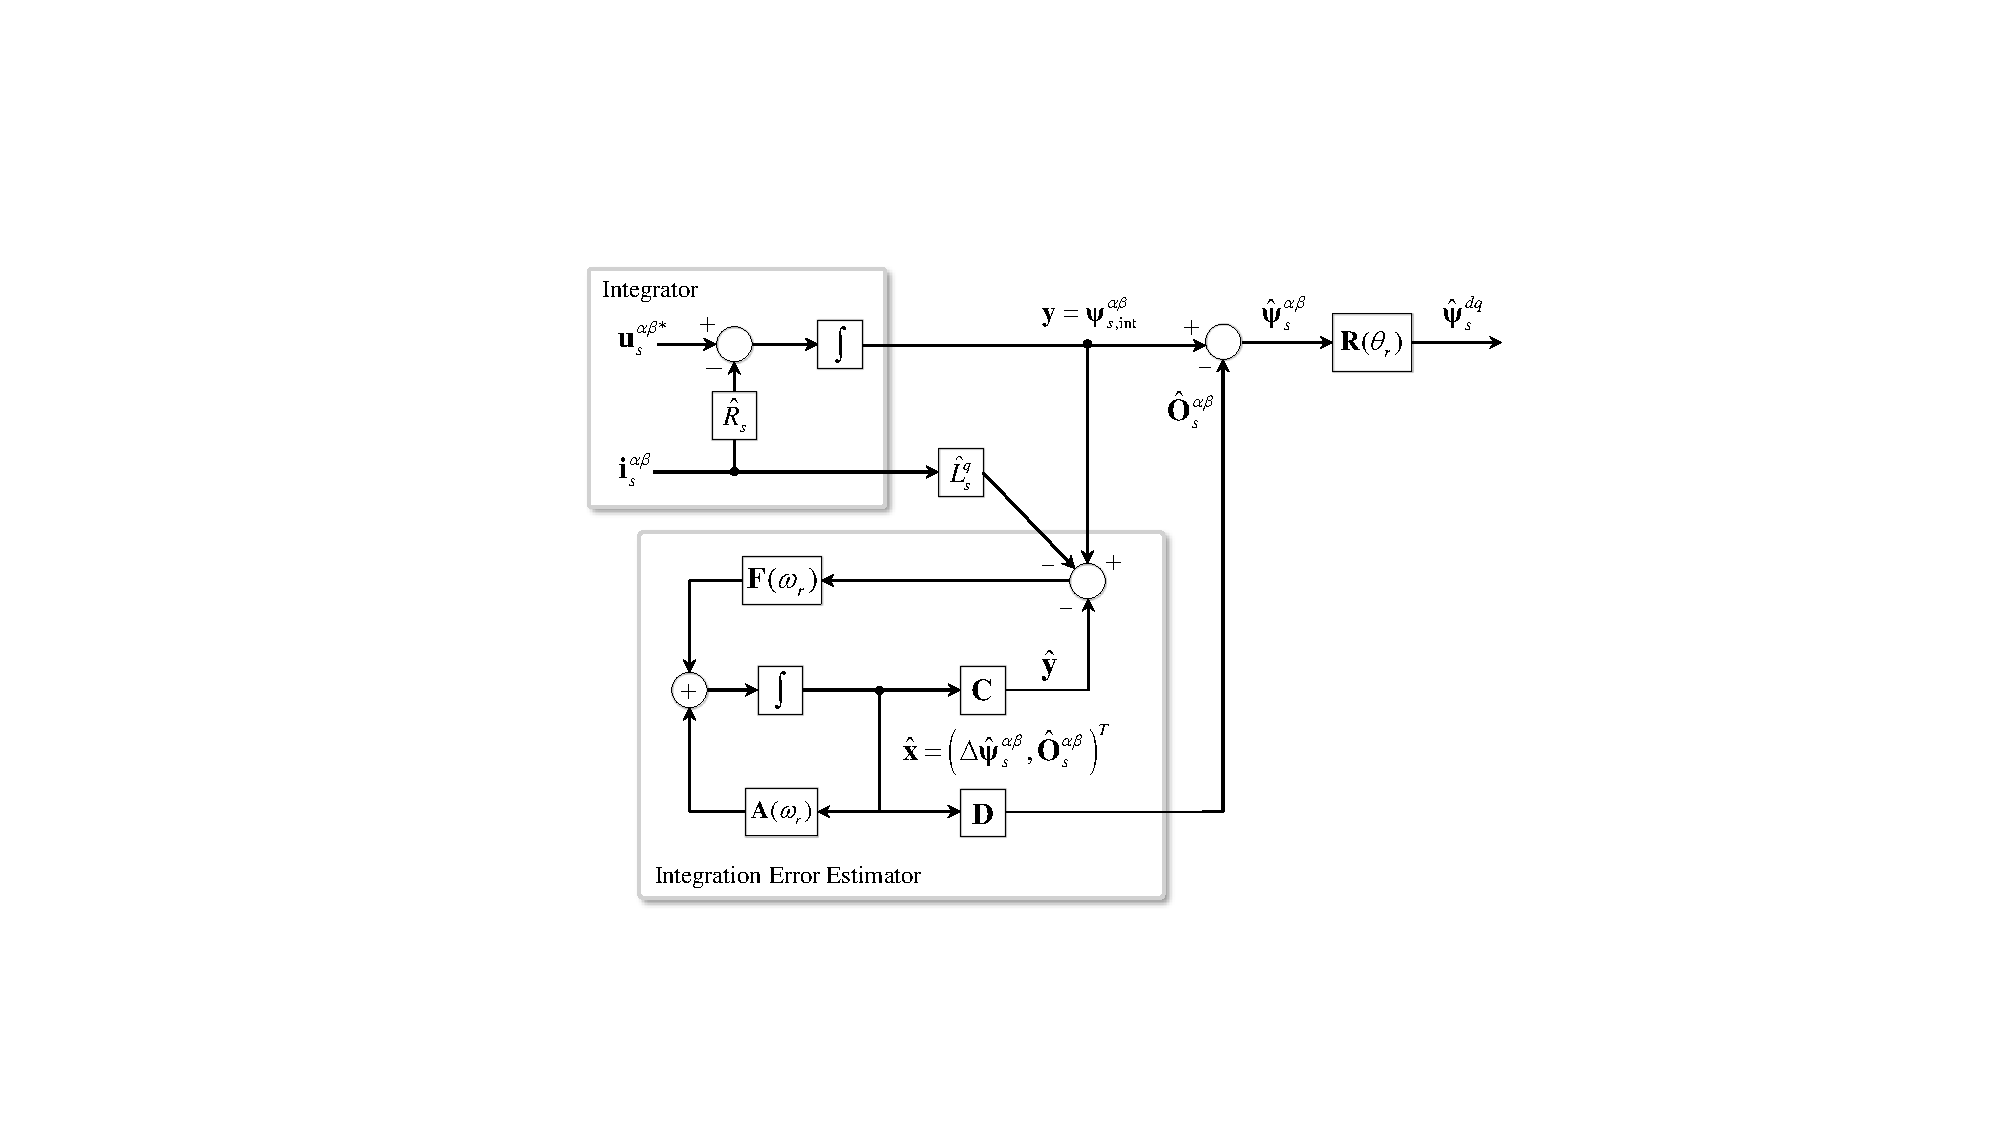
\includegraphics[scale=0.8]{chapters/Fig3.2.pdf}
    \caption{Proposed stator flux linkage estimator based on the integration error estimator}
    \label{Fig:3.2}
\end{figure}

Finally, the estimate of the stator flux linkage vector \( \boldsymbol{\hat{\psi}}^{\alpha\beta}_s \) in the (\(\alpha\),\(\beta\))-reference frame can be obtained by subtracting the integration error estimate \( \boldsymbol{\hat{O}}^{\alpha\beta}_s \) from the integration result \( \boldsymbol{\hat{\psi}}^{\alpha\beta}_{s,\text{int}} \), i.e.
\begin{align}\notag
\boldsymbol{\hat{\psi}}^{\alpha\beta}_s(t) &= \boldsymbol{\hat{\psi}}^{\alpha\beta}_{s,\text{int}}(t) - \boldsymbol{\hat{O}}^{\alpha\beta}_s(t) \\\label{eqn:3.15}
&= \mathbf{y}(t) - \mathbf{D} \boldsymbol{\hat{x}}(t),
\end{align}
with $\mathbf{D} := [\mathbf{O}_{2\times2} \quad \mathbf{I}_{2\times2} ]$. By applying the coordinate transformation in (\ref{eqn:2.8}) to the (\(\alpha,\beta\))-axis estimates in (\ref{eqn:3.15}), the flux estimates in the ($d$,$q$)-reference frame can be obtained as follows
\begin{equation}\label{eqn:3.16}
\boldsymbol{\hat{\psi}}^{dq}_s(t) = \mathbf{R}(\theta_r) \boldsymbol{\hat{\psi}}^{\alpha\beta}_s(t).
\end{equation}

\subsection{Parameter Update for Improving Transient Estimation Performance}
Recalling (\ref{eqn:3.8}) and Assumption (A.3.1), the transient estimation performance of (\ref{eqn:3.16}) depends on the accuracy of the $q$-axis inductance parameter used in the observer of (\ref{eqn:3.13}). Therefore, if the parameter inaccuracy increases, the magnitude of \(\tilde{L}_q\) in (\ref{eqn:3.8}) increases, leading to a larger disturbance vector \(\mathbf{d}^{\alpha\beta,\psi}_s\), which ultimately degrades transient estimation performance. Thus, it is necessary to estimate the $q$-axis inductance online based on the stator current and update it to the actual value to improve transient estimation performance. 

\subsubsection{Parameter Identification Using a Recursive Least-Square Method}
To estimate the parameters online, the Recursive Least Squares (RLS) method with a forgetting factor for continuous time, which is robust to signal noise and inaccuracies, is generally applied \cite{c3.2_4}. For parameter identification, the linear parametric model for the $q$-axis flux linkage can be expressed as
\begin{equation}\label{eqn:3.17}
    \psi^q_s(t) = L^q_s(t)i^q_s(t), \quad \hat\psi^q_s(t) \rightarrow \psi^q_s(t) \text{ as t } \rightarrow \infty,
\end{equation}
where the flux estimate \(\hat \psi^q_s\) is used as the output of the linear parametric model since the $q$-axis flux linkage \(\psi^q_s\) cannot be directly measured (the estimation error \(\mathbf{\tilde{x}}\) asymptotically converges to the zero vector \(\mathbf{O}_2\) as \(t \rightarrow \infty\)). To estimate the unknown $q$-axis inductance parameter, the linear model in (\ref{eqn:3.17}) is rearranged as follows
\begin{equation}\label{eqn:3.18}
\begin{aligned}
z &= \theta^* u = \hat\psi^q_s(t), \ \theta^* = L^q_s(t), \ u = i^{q}_s(t),
\end{aligned}
\end{equation}
where \(z\) represents the output signals of the parametric model, \(\theta^*\) is the unknown parameter to be estimated, and \(u\) represents the input signals, respectively. The estimate of $z$ in (\ref{eqn:3.18}) can be expressed as  
\begin{equation}\label{eqn:3.19}
\hat{z} = \theta u, \ \theta = \hat{L}^q_s(t),
\end{equation}
where \(\hat{z}\) and \(\theta\) denote the estimate of \(z\) and the estimated parameter of \(\theta^*\), respectively and the parameter estimation error
\begin{equation}\label{eqn:3.20}
\epsilon =z - \hat{z} = z - \theta u
\end{equation}
can be derived. Therefore, to minimize the parameter estimation error in (\ref{eqn:3.20}) and identify the parameter $\theta$ using a convex integral objective function, the continuous-time recursive least-squares parameter update algorithm (see Appendix \ref{Appen1})
\begin{equation}\label{eqn:3.21}
\begin{aligned}
\dot{\theta} &= \Gamma \epsilon^\top u \\
    \dot{\Gamma} &= \beta \Gamma - \Gamma u^\top u \Gamma
\end{aligned}
\end{equation}
with the covariance $\Gamma$ and the forgetting factor $\beta$. Therefore, if the input signal \(u\) satisfies the PE (Persistent Excitation) condition and \(\theta\) and \(\dot{\theta}\) are uniformly bounded, then \(\theta\) will eventually converge exponentially to the actual parameter \(\theta^*\). Therefore, by using the RLS algorithm in (\ref{eqn:3.21}) to update the $q$-axis inductance parameter in the observer of (\ref{eqn:3.13}) online, the transient estimation performance can be improved.

\subsubsection{Adaptive Observer based on the Parameter Update}
The flux estimation error made by the inductance parameter (\(\hat{L}^q_s\)) update in (\ref{eqn:3.21}) can be compensated for by an adaptive observer that adds an auxiliary term to the flux estimation dynamics. The $\alpha$-$\beta$ axis rotating nonlinear flux linkage vector $\Delta \boldsymbol{\psi}^{\alpha \beta}_s$ in (\ref{eqn:3.6a}) can be redefined as
\begin{align}\label{eqn:3.23}
\boldsymbol{\psi}^{\alpha\beta}_s(t) = L^q_s(t) \mathbf{i}^{\alpha\beta}_s(t) + 
\underbrace{\mathbf{P}(\theta_r)
\Delta \psi^{d}_s(t)}_{=:\Delta \boldsymbol{\psi}^{\alpha \beta}_s(t)},
\end{align}
where the time derivative of the rotating nonlinear flux in (\ref{eqn:3.23}) leads
\begin{equation}\label{eqn:3.24}
\begin{aligned}
\frac{d}{dt}{\boldsymbol{\Delta \psi}}^{\alpha\beta}_s(t) &= \omega_r(t) \mathbf{J}\underbrace{\mathbf{P}(\theta_r)\Delta \psi^{d}_s(t)}_{\stackrel{(\ref{eqn:3.23})}=\Delta\boldsymbol{\psi}^{\alpha\beta}_s}+\underbrace{\mathbf{P}(\theta_r) \Delta \dot\psi^{ d}_s(t)}_{=:\mathbf{d}^{\alpha\beta,\psi}_{s}(t)}
\\
&= \omega_r(t) \mathbf{J} \Delta \boldsymbol{\psi}^{\alpha\beta}_s(t) + \mathbf{d}^{\alpha\beta,\psi}_{s}(t)
\end{aligned},
\end{equation}
where the disturbance vector \(\mathbf{d}^{\alpha\beta,\psi}_s\) converges to zero in steady state, recalling Assumption (A.2.2). Accordingly, the output ($\boldsymbol{\psi}^{\alpha\beta}_{s,\text{int}}$) and dynamics ($\Delta \dot{\boldsymbol{\psi}}^{\alpha \beta}_s$,$\dot{\mathbf{O}}^{\alpha\beta}_s$) are summarized as follows
\begin{equation}
\begin{aligned}\label{eqn:3.25}
\begin{cases}
\frac{d}{dt}{\Delta \boldsymbol{\psi}}^{\alpha\beta}_s(t) = \omega_r(t) \mathbf{J} \Delta \boldsymbol{\psi}^{\alpha\beta}_s(t) + \mathbf{d}^{\alpha\beta,\psi}_{s}(t) \\
\frac{d}{dt}{\mathbf{O}}^{\alpha\beta}_s(t) = \mathbf{d}^{\alpha\beta,o}_{s}(t) \\
\boldsymbol{\psi}^{\alpha\beta}_{s,\text{int}}(t) = L^q_s(t) \mathbf{i}^{\alpha\beta}_s(t) + 
\Delta \boldsymbol{\psi}^{\alpha \beta}_s(t) + \mathbf{O}^{\alpha\beta}_s(t)
\end{cases}
\end{aligned},
\end{equation}
where the state-space model in (\ref{eqn:3.25}) is the same as (\ref{eqn:3.11}) except for \(\theta := L^q_s\). Thus, an adaptive observer 
\begin{equation}\label{eqn:3.26}
\left\{
\begin{aligned}
    \frac{d}{dt} \hat{\mathbf{x}}(t) &= \mathbf{A}(\omega_r) \hat{\mathbf{x}} + \mathbf{F}(\omega_r) \left( \mathbf{y}(t) - \mathbf{C} \hat{\mathbf{x}}(t) - \mathbf{\Psi}(t) \hat\theta(t) \right) + \mathbf{w}(t) \\
    \hat{\mathbf{y}}(t) &= \mathbf{C} \hat{\mathbf{x}}(t) + \mathbf{\Psi}(t) \hat{\theta}(t)
\end{aligned}
\right.
\end{equation}
can be designed, where \(\theta := L_q\) is an unknown actual inductance parameter and \(\mathbf{w}\) is an auxiliary term in order to compensate the estimation error made by parameter estimate $\hat\theta$. Since there are no changes in the \( \mathbf{A}(\omega_r) \) and \( \mathbf{C} \) matrices, the rank of the observability matrix remains the same in (\ref{eqn:3.11}), ensuring that all states can be observed. By subtracting (\ref{eqn:3.11}) from  (\ref{eqn:3.26}), the estimation error dynamics
\begin{equation}\label{eqn:3.27}
\frac{d}{dt} \tilde{\mathbf{x}}(t) = \left[ \mathbf{A}(\omega_r) - \mathbf{F}(\omega_r)\mathbf{C} \right] \tilde{\mathbf{x}}(t) - \mathbf{F}(\omega_r)\mathbf{\Psi}(t) \tilde\theta(t) + \mathbf{w}(t) - {\mathbf{d}_{t}}(t)
\end{equation}
with the parameter estimation error \(\tilde{\theta} := \hat{\theta} - \theta\). To design an adaptation law that compensates for the term \(\mathbf{F}(\omega_r)\mathbf{\Psi}\tilde\theta\), which affects the convergence of the estimation error dynamics in (\ref{eqn:3.27}) due to parameter estimation error, with an auxiliary term \(\mathbf{w}\), the following assumption is introduced \cite{c3.2_5}.

\textbf{Assumption (A.3.4)} The state estimation error \(\tilde{\mathbf{x}}\), parameter estimation error \(\tilde{\theta}\), and the time-varying matrix \(\boldsymbol{\Upsilon}\) can be expressed as a linear combination of \(\boldsymbol{\eta}\) \cite{c3.2_6} as follows
\begin{equation}\label{eqn:3.28}
\boldsymbol{\eta}(t) = \tilde{\mathbf{x}}(t) - \boldsymbol{\Upsilon}(t) \tilde{\theta}(t),
\end{equation}

Considering Assumption (A.3.4), the time derivative of (\ref{eqn:3.28}) can be expressed as 
\begin{align}\label{eqn:3.29}
\frac{d}{dt}{\boldsymbol{\eta}}(t) &= \dot{\tilde{\mathbf{x}}}(t) - \mathbf{\Upsilon}(t) \dot{\tilde{\theta}}(t) - \dot{\mathbf{\Upsilon}}(t) \tilde{\theta}(t) \\\notag
&= \underbrace{(\mathbf{A}(\omega_r) - \mathbf{F}(\omega_r)\mathbf{C})}_{:= \mathbf{A}_c} \tilde{\mathbf{x}}(t) - \mathbf{F}(\omega_r)\mathbf{\Psi}(t) \tilde{\theta}(t) +\mathbf{w}(t) - {\mathbf{d}_{t}}(t) 
-\mathbf{\Upsilon} \dot{\tilde{\theta}}(t) - \dot{\mathbf{\Upsilon}} \tilde{\theta}(t) \\\notag
&= \mathbf{A}_c {\boldsymbol{\eta}}(t)+ \left[ \mathbf{A}_c \mathbf{\Upsilon}(t) - \mathbf{F}(\omega_r)\mathbf{\Psi}(t) - \dot{\mathbf{\Upsilon}}(t) \right] \tilde{\theta}(t) + \mathbf{w}(t) - \mathbf{\Upsilon}(t) \dot{\tilde{\theta}}(t) 
- {\mathbf{d}_{t}}(t)
\end{align}
where \(\dot{\theta}\) becomes zero as \( t \rightarrow \infty \). Therefore, to make the equation in (\ref{eqn:3.29}) stable, the \(\tilde{\theta}\) and \(\dot{\tilde{\theta}}\) terms can be eliminated by
\begin{equation}\label{eqn:3.30}
\begin{aligned}
\dot{\mathbf{\Upsilon}}(t) &= \mathbf{A}_c \mathbf{\Upsilon}(t) - \mathbf{F}(\omega_r) \mathbf{\Psi}(t)\\
    \mathbf{w}(t) &= \mathbf{\Upsilon}(t) \dot{\tilde{\theta}}(t)=\mathbf{\Upsilon}(t)\dot{\hat{\theta}}(t)
\end{aligned},
\end{equation}
where the equation in (\ref{eqn:3.29}) can be rearranged as 
\begin{align}\label{eqn:3.31}
\dot{\boldsymbol{\eta}}(t) &=  \mathbf{A}_c \boldsymbol{\eta}(t) 
- {\mathbf{d}_{t}}(t).
\end{align}
If the observer matrix \(\mathbf{A}_c\)  becomes Hurwitz (stable) and under Assumption (A.2.2) and Assumption (A.3.3) (${\mathbf{d}_{t}}\rightarrow 0$ as $ t \rightarrow \infty$) in steady state, \(\boldsymbol{\eta}\) is exponentially stable, resulting in \(\hat{x} \rightarrow x\) and \(\hat{\theta} \rightarrow \theta\). The adaptive algorithm for the adaptive observer based on the parameter update is summarized as follows
\begin{equation}\label{eqn:3.34}
\left\{
\begin{aligned}
\dot{\mathbf{\Upsilon}}(t) &= \mathbf{A}_c \mathbf{\Upsilon}(t) - \mathbf{F}(\omega_r) \mathbf{\Psi}(t)\\
    \mathbf{w}(t) &=\mathbf{\Upsilon}(t)\dot{\hat{\theta}}(t)
    \\
        \dot{\hat\theta} &= \Gamma \epsilon^\top u\\
    \dot{\Gamma} &= \beta \Gamma - \Gamma u^\top u \Gamma
\end{aligned},
\right.
\end{equation}
with
\begin{equation*}
z = \hat\psi^q_s(t),\quad u = i^q_s, \quad \hat{\theta} = \hat{L}^q_s(t) , \quad \epsilon =z - \hat{\theta}u.
\end{equation*}

Therefore, the proposed adaptive observer compensates for the flux estimation error caused by the inductance parameter error estimated by RLS by adding an auxiliary term \(\mathbf{w}\) to the estimation dynamics through an adaptation law. This approach reduces the norm of the disturbance vector \(\|\mathbf{d}^{\alpha\beta,\psi}_s\|\), improving transient estimation performance and ensuring robustness against parameter variations in the observer.